%%
%% This is file `sample-manuscript.tex',
%% generated with the docstrip utility.
%%
%% The original source files were:
%%
%% samples.dtx  (with options: `manuscript')
%% 
%% IMPORTANT NOTICE:
%% 
%% For the copyright see the source file.
%% 
%% Any modified versions of this file must be renamed
%% with new filenames distinct from sample-manuscript.tex.
%% 
%% For distribution of the original source see the terms
%% for copying and modification in the file samples.dtx.
%% 
%% This generated file may be distributed as long as the
%% original source files, as listed above, are part of the
%% same distribution. (The sources need not necessarily be
%% in the same archive or directory.)
%%
%% Commands for TeXCount
%TC:macro ~\cite [option:text,text]
%TC:macro ~\citep [option:text,text]
%TC:macro ~\citet [option:text,text]
%TC:envir table 0 1
%TC:envir table* 0 1
%TC:envir tabular [ignore] word
%TC:envir displaymath 0 word
%TC:envir math 0 word
%TC:envir comment 0 0
%%
%%
%% The first command in your LaTeX source must be the \documentclass command.
%%%% Small single column format, used for CIE, CSUR, DTRAP, JACM, JDIQ, JEA, JERIC, JETC, PACMCGIT, TAAS, TACCESS, TACO, TALG, TALLIP (formerly TALIP), TCPS, TDSCI, TEAC, TECS, TELO, THRI, TIIS, TIOT, TISSEC, TIST, TKDD, TMIS, TOCE, TOCHI, TOCL, TOCS, TOCT, TODAES, TODS, TOIS, TOIT, TOMACS, TOMM (formerly TOMCCAP), TOMPECS, TOMS, TOPC, TOPLAS, TOPS, TOS, TOSEM, TOSN, TQC, TRETS, TSAS, TSC, TSLP, TWEB.
% \documentclass[acmsmall]{acmart} 

%%%% Large single column format, used for IMWUT, JOCCH, PACMPL, POMACS, TAP, PACMHCI
% \documentclass[acmlarge,screen]{acmart}

%%%% Large double column format, used for TOG
% \documentclass[acmtog, authorversion]{acmart}

%%%% Generic manuscript mode, required for submission
%%%% and peer review
\documentclass[manuscript,screen,review]{acmart}


\usepackage{todonotes}
\usepackage{multirow}
\usepackage{enumitem}
\usepackage{ragged2e}
\usepackage{graphicx}
\usepackage{hyperref}
\usepackage{cleveref}
\usepackage{ulem}
\usepackage{tabto}
\graphicspath{ {./images/} }

%% Fonts used in the template cannot be substituted; margin 
%% adjustments are not allowed.
%%
%% \BibTeX command to typeset BibTeX logo in the docs
\AtBeginDocument{%
  \providecommand\BibTeX{{%
    \normalfont B\kern-0.5em{\scshape i\kern-0.25em b}\kern-0.8em\TeX}}}

%% Rights management information.  This information is sent to you
%% when you complete the rights form.  These commands have SAMPLE
%% values in them; it is your responsibility as an author to replace
%% the commands and values with those provided to you when you
%% complete the rights form.
\setcopyright{acmlicensed}
\copyrightyear{2024}
\acmYear{2026}
\acmDOI{XXXXXXX.XXXXXXX}

%% These commands are for a PROCEEDINGS abstract or paper.
% \acmConference[Conference acronym 'XX]{Make sure to enter the correct conference title from your rights confirmation email}{June 03--05, 2018}{Woodstock, NY}
\acmConference[JMUHT '25]{JMU Honor's Thesis in Computer Science 2025}{May 2025}{Harrisonburg, Virginia}
%
%  Uncomment \acmBooktitle if th title of the proceedings is different
%  from ``Proceedings of ...''!
%
% \acmBooktitle{Woodstock '18: ACM Symposium on Neural Gaze Detection, June 03--05, 2018, Woodstock, NY} 
\acmISBN{978-1-4503-XXXX-X/18/06}


%%
%% Submission ID.
%% Use this when submitting an article to a sponsored event. You'll
%% receive a unique submission ID from the organizers
%% of the event, and this ID should be used as the parameter to this command.
%%\acmSubmissionID{123-A56-BU3}

%%
%% For managing citations, it is recommended to use bibliography
%% files in BibTeX format.
%%
%% You can then either use BibTeX with the ACM-Reference-Format style,
%% or BibLaTeX with the acmnumeric or acmauthoryear sytles, that include
%% support for advanced citation of software artefact from the
%% biblatex-software package, also separately available on CTAN.
%%
%% Look at the sample-*-biblatex.tex files for templates showcasing
%% the biblatex styles.
%%

%%
%% The majority of ACM publications use numbered citations and
%% references.  The command ~\citestyle{authoryear} switches to the
%% "author year" style.
%%
%% If you are preparing content for an event
%% sponsored by ACM SIGGRAPH, you must use the "author year" style of
%% citations and references.
%% Uncommenting
%% the next command will enable that style.
%%~\citestyle{acmauthoryear}

%%
%% end of the preamble, start of the body of the document source.
\begin{document}
%%
%% The "title" command has an optional parameter,
%% allowing the author to define a "short title" to be used in page headers.
\title{Beats, Bytes, and Belonging: Fostering Identity and Inclusion through the Digital Audio Workstation}

%%
%% The "author" command and its associated commands are used to define
%% the authors and their affiliations.
%% Of note is the shared affiliation of the first two authors, and the
%% "authornote" and "authornotemark" commands
%% used to denote shared contribution to the research.
\author{Matthew F. Wolffe}
\email{wolffemf@dukes.jmu.edu}
\orcid{0009-0009-1072-00132}
% with a committee section in place, I need not be an official author of the doc.
% \author{Michael C. Stewart}
% \email{stewarmc@jmu.edu}
% \orcid{0000-0002-8833-7833}
\affiliation{%
  \institution{James Madison University}
  \streetaddress{701 Carrier Dr.}
  \city{Harrisonburg}
  \state{Virginia}
  \country{USA}
  \postcode{22807}
}

%%
%% By default, the full list of authors will be used in the page
%% headers. Often, this list is too long, and will overlap
%% other information printed in the page headers. This command allows
%% the author to define a more concise list
%% of authors' names for this purpose.
% \renewcommand{\shortauthors}{Wolffe and Stewart}
% \renewcommand{\shortauthors}{Wolffe}

%%
%% The code below is generated by the tool at http://dl.acm.org/ccs.cfm. % TODO: Matt
%% Please copy and paste the code instead of the example below.
%%
\begin{CCSXML}
<ccs2012>
   <concept>
       <concept_id>10003120.10003121.10003124.10010868</concept_id>
       <concept_desc>Human-centered computing~Web-based interaction</concept_desc>
       <concept_significance>300</concept_significance>
       </concept>
   <concept>
       <concept_id>10003120.10003121.10003124.10010865</concept_id>
       <concept_desc>Human-centered computing~Graphical user interfaces</concept_desc>
       <concept_significance>100</concept_significance>
       </concept>
   <concept>
       <concept_id>10003120.10003121.10003125.10010597</concept_id>
       <concept_desc>Human-centered computing~Sound-based input / output</concept_desc>
       <concept_significance>300</concept_significance>
       </concept>
   <concept>
       <concept_id>10010405.10010489.10010491</concept_id>
       <concept_desc>Applied computing~Interactive learning environments</concept_desc>
       <concept_significance>500</concept_significance>
       </concept>
   <concept>
       <concept_id>10010405.10010489.10010492</concept_id>
       <concept_desc>Applied computing~Collaborative learning</concept_desc>
       <concept_significance>100</concept_significance>
       </concept>
   <concept>
       <concept_id>10010405.10010489.10010493</concept_id>
       <concept_desc>Applied computing~Learning management systems</concept_desc>
       <concept_significance>500</concept_significance>
       </concept>
   <concept>
       <concept_id>10010405.10010489.10010490</concept_id>
       <concept_desc>Applied computing~Computer-assisted instruction</concept_desc>
       <concept_significance>300</concept_significance>
       </concept>
   <concept>
       <concept_id>10010405.10010469.10010471</concept_id>
       <concept_desc>Applied computing~Performing arts</concept_desc>
       <concept_significance>500</concept_significance>
       </concept>
   <concept>
       <concept_id>10010405.10010469.10010474</concept_id>
       <concept_desc>Applied computing~Media arts</concept_desc>
       <concept_significance>300</concept_significance>
       </concept>
   <concept>
       <concept_id>10010405.10010469.10010475</concept_id>
       <concept_desc>Applied computing~Sound and music computing</concept_desc>
       <concept_significance>500</concept_significance>
       </concept>
 </ccs2012>
\end{CCSXML}

\ccsdesc[300]{Human-centered computing~Web-based interaction}
\ccsdesc[100]{Human-centered computing~Graphical user interfaces}
\ccsdesc[300]{Human-centered computing~Sound-based input / output}
\ccsdesc[500]{Applied computing~Interactive learning environments}
\ccsdesc[100]{Applied computing~Collaborative learning}
\ccsdesc[500]{Applied computing~Learning management systems}
\ccsdesc[300]{Applied computing~Computer-assisted instruction}
\ccsdesc[500]{Applied computing~Performing arts}
\ccsdesc[300]{Applied computing~Media arts}
\ccsdesc[500]{Applied computing~Sound and music computing}


%%
%% Keywords. The author(s) should pick words that accurately describe
%% the work being presented. Separate the keywords with commas.
\keywords{Human Computer Interaction, Instrumental Music Education, Digital Audio Workstation, Web Development, DEI in Music Education, Full-stack development, Modern Band, Technological Literacy}

%% A "teaser" image appears between the author and affiliation
%% information and the body of the document, and typically spans the
%% page.
% \begin{teaserfigure}
%   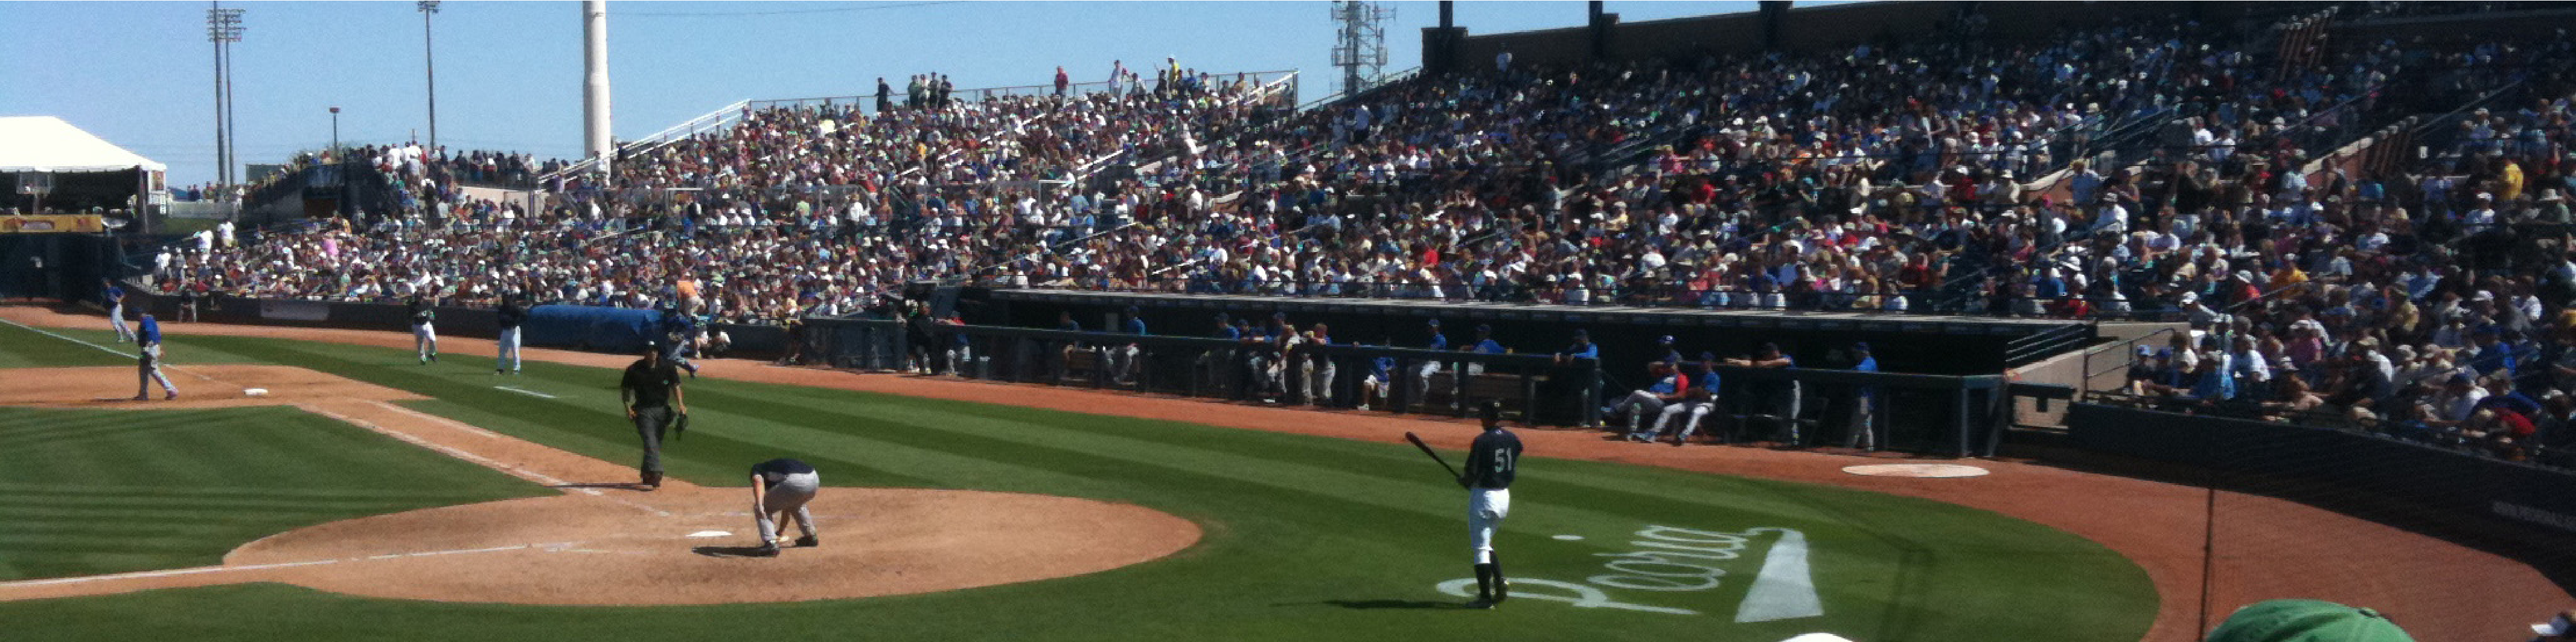
\includegraphics[width=\textwidth]{sampleteaser}
%   \caption{Seattle Mariners at Spring Training, 2010.}
%   \Description{Enjoying the baseball game from the third-base
%   seats. Ichiro Suzuki preparing to bat.}
%   \label{fig:teaser}
% \end{teaserfigure}

% \received{20 February 2007}
% \received[revised]{12 March 2009}
% \received[accepted]{5 June 2009}

%%
%% This command processes the author and affiliation and title
%% information and builds the first part of the formatted document.
\maketitle

% https://authors.acm.org/proceedings/production-information/preparing-your-article-with-latex

\section*{Committee}
\def\dotsign{\xleaders\hbox to .2em{\d{}}\hfill\d{}}
\def\dashsign{\xleaders\hbox to .5em{\_}\hfill\_}

\begin{centering}
\tabcolsep0pt
\begin{tabular}{lp{.5\linewidth}@{}}
Approved:~ & \\[-3pt]\cmidrule{2-2} 
& Michael Stewart, Ph.D., \textbf{Chair}\\
& Associate Professor, Computer Science\\
\end{tabular}

\tabcolsep0pt
\begin{tabular}{lp{.5\linewidth}@{}}
Approved:~ & \\[-3pt]\cmidrule{2-2} 
& Chris Johnson, Ph.D.\\
& Associate Professor, Computer Science\\
\end{tabular}

\tabcolsep0pt
\begin{tabular}{lp{.5\linewidth}@{}}
Approved:~ & \\[-3pt]\cmidrule{2-2} 
& Dee A. B. Weikle, Ph.D.\\
& Professor, Computer Science\\
\end{tabular}

\end{centering}


\section*{Proposal}
I propose to integrate a basic Digital Audio Workstation (DAW) into an existing niche Learning Management System for instrumental music education (IME) to study research questions in Human Computer Interaction (HCI) related to the impact of the DAW on students' musical self-efficacy and identities, creative thinking, and feelings of belonging in the IME classroom.

In addition, I propose that a pilot study be carried out in advance of the primary research in order to examine questions of user design, experience, and impact. Namely, whether access to the DAW is conducive to student submission quality and may someday act as a bridge from IME to digital music education by building user agency and technological literacy, while also reducing strain on instructors.  

\pagebreak

\section{Introduction} 
Instrumental Music Education (IME) programs in the United States have been in gradual decline for the last 40 years, in part due to bureaucratic incongruities regarding what constitutes student success and the subsequent budgetary tug-of-war~\cite{Lehman20}, but also in response to dissonance between a reluctance to expand the canon and broadening student interests and identities~\cite{Vasil23}. Music education at the middle and high school levels largely adheres to the Western European Canon (WEC) with respect to instrumentation and repertoire.
Music both from and inspired by this genre is often colloquially referred to as, `the music of dead white men', so it comes as no surprise that 21\textsuperscript{st} century students feel disconnected from the standard repertoire by time, geography, and culture.

Like many other fields of study, IME struggles with issues of exclusivity.
The instruments of the WEC can be prohibitively expensive---even `student model' instruments can cost thousands of dollars. 
Because of these costs, band programs rarely have funds to replace decades-old instruments.
In addition, for those students who enjoy playing and performing on their instrument, private instruction is commonly needed for them to advance to an appropriate skill level for competitions and college auditions.
However, weekly lessons with experienced private teachers can be expensive.
To make matters worse, if a student aspires to play in a professional orchestra, they and their families will likely be dismayed to learn that for many instruments, there is an unwritten expectation that professional players own and have mastered several variants of their instrument before auditioning.
For example, the tubist of any given major symphony orchestra in the United States is often expected to have both F bass and C contrabass tubas at their disposal.
Furthermore, these expectations vary by country. In Germany for instance, a principal tubist is expected to play F bass and B$\flat$ contrabass;
in the UK, E$\flat$ bass and C contrabass;
in Holland, E$\flat$ bass and B$\flat$ contrabass are the custom.
Unfortunately, these cost barriers and the disconnect with respect to the WEC disproportionately affect minorities. 

It is worth noting that historically, barriers to entry to participation in the WEC were created and institutionalized intentionally, rather than evolving from naive and perfunctory abidance by precedent.
% consider a well-established, well-resourced, highly celebrated, well-respected orchestra (VPO)
% to demonstrate/iullustrate intentionality, even after adopting a progressive practice that arguably prioritized musicianship/expertise in which <blind audition> and seeing reduced bias in selectoin, the orchestra anyway chose to discontinue the practice because of bigoted backlash from its members/leadership.
To illustrate, the Vienna Philharmonic Orchestra (VPO) is known today as one of the leading orchestras of the world, however it has an extensive history of intentionally exclusionary practices.  Following the Second World War, in an effort to promote unbiased judgment of auditioners, the VPO joined a growing trend in which orchestras instituted blind auditions.
% possibly problematic use of the word blinf in today's cultural context, but very likely the citable term fore this practice...Weikle agrees
Unfortunately, leaders of the VPO protested this practice, and subsequently changed audition procedures so that applicants could be seen in the final round and dismissed if not white~\cite{VPO-corollary}. Illustrating the more common position of the VPO, during a 1996 broadcast, then-chairman of the VPO Werner Resel answered a visiting female student's question about why all musicians in the orchestra were male by asserting that the ``Vienna Philharmonic is an orchestra of white men playing music by white men for white people''~\cite{VPO-corollary}.

While a legacy of discrimination is undeniable, new technologies may help us eliminate prejudice-borne barriers to entry.
Music as a whole, as with most fields of study, saw striking shifts in performance and practice in parallel with the technological leaps of the 20\textsuperscript{th} century~\cite{Katz10}.
For the musical arts, these technological leaps had a side-effect of blurring the lines between practice, performance, notation, and consumption.
With digitization came the development of highly robust and powerful software that, in one or two packages, can perform an impressive breadth of musical roles and tasks.
For instance, using Avid Technology’s DAW, Pro Tools~\cite{ProTools}, and their engraving software, Sibelius~\cite{Sibelius} allows for the efficient creation of highly complex musical works, whether by mouse and keyboard or recorded sonic input.
From here a user can choose to generate virtual instrument playback, and can then mix, master, edit, and extend upon their initial composition, all of which are often done today as part of a live performance---it is not uncommon to see a laptop alongside a performer on stage. 

The technologies described above constitute part of a larger `hidden curriculum' of 21\textsuperscript{st} century music education. 
For many people, even those pursuing WEC-oriented careers, progressing in any musical endeavor --- professional or otherwise --- may require they be able to mix, master, and publish their own music.
In other words, it requires they demonstrate enough technological literacy to efficiently operate (often complex) software that can perform these tasks.
Considering that these technologies are not traditionally taught in IME programs, if a student is made aware of and hopes to learn these skills, they must do so independent of their IME classes.
In addition to digital audio technologies, there is a stark lack of instruction on creative musical tasks such as voice-leading, arranging, improvising, and practicing extended techniques on instruments.
Unfortunately, students often do not receive formal training in these creative tasks unless they choose to study music at the university level.

To combat declining interest and participation in IME, some teachers throughout the United States would like to embrace or have already embraced technology by trying to incorporate ``modern band'' into their curricula~\cite{Dammers}.
Modern band is an approach to music education that adheres to a different canon: popular music from contemporary genres such as rock, hip-hop, and electronic dance music.
For students in these programs, modern band has not only improved engagement and motivation, but also helped to increase the depth of their musical and technical fluency, build community, form friendships, and foster creativity and exploration of musical identity~\cite{Vasil23}.
The program has found success in attracting students across the board~\cite{NelsonKelly}, and particularly in students coming from more diverse backgrounds in terms of race and ethnicity~\cite{Vasil23}.

Unfortunately, instructors who adopt modern band into the existing curriculum encounter many obstacles.
Music educators often lack experience with respect to genres and techniques outside the WEC ---
this particular issue has been noted as early as the 1967 Tanglewood Symposium~\cite{Lehman20, Vasil23}.
Further, it's common for those who are brought up and trained on the standard repertoire to remain deadlocked in ivory towers by bias against popular music~\cite{ClauhsSanguinetti}, or dissuaded from exploring nontraditional genres by poor technological literacy~\cite{Bannerman}.
For open-minded teachers already spread too thin, finding the time for tasks unique to preparing a modern band classroom---procuring nontraditional instruments, screening and adapting lyrics, arranging and transcribing student selected music, and more---can be incredibly taxing~\cite{Vasil23}. 

I propose to contribute to the efforts to increase student engagement and feelings of belonging in the IME classroom and facilitate instructors' adoption of ``modern band'' by expanding the existing IME learning management system, MusicCPR, to include a simple digital audio workstation.


\section{The M\MakeLowercase{usic}CPR Platform}
Like other teachers, instrumental music educators are over-tasked and under-resourced, possibly to a greater extent than instructors in other fields due to the shrinking budgets and greater priority given to other fields.
% (while some subjects' budgets have ballooned, e.g. STEM)
Further, there is a particularly large theory-practice gap within music education; that is, research findings rarely make their way to practice.

MusicCPR, a free and open source web platform which aims to mitigate the above challenges, is a collaborative effort between James Madison University, the Eastman School of Music of the University of Rochester, and the University of Delaware's School of Music. 
Our primary motivations so far have been: (1) facilitating individual performance assessment, and (2) closing the theory-practice gap with activities designed to capture the artistic processes enumerated in the National Core Arts Standards: Create, Perform, Respond, and Connect~\cite{core_arts, CPR}.

Ideally, widespread adoption of MusicCPR by schools would also help to chip away at issues of exclusivity in IME, namely the following:
\begin{itemize}
    \item Relevance, in terms of:
    \begin{itemize}
        \item Local geography
        \item Student identities, e.g., cultural backgrounds and listening habits
    \end{itemize}
    \item Cost
    \begin{itemize}
        \item Purchase and maintenance of instruments
        \item Private instruction 
    \end{itemize}
    \item Technological literacy
    \begin{itemize}
        \item In the 21st century, proficiency with certain technologies is essentially a requirement for music sharing, publishing, and to some extent, collaboration with other musicians. 
    \end{itemize}
\end{itemize}

\section{Justification and Purpose}
We intend to build a simple digital audio workstation within MusicCPR.
While there are many different types of music software that may be integrated within MusicCPR in relatively little time, we selected a DAW for the following reasons:

\begin{itemize}
    \item Prior research has shown that middle and high school students are interested in using DAWs for musical composition~\cite{PendergastRobinson}.
    \item MusicCPR already makes use of the online music notation application, Flat~\cite{Flat}.
    \item DAWs can perform an extensive variety of different functions.
    \begin{itemize}
        \item Thanks to this variety, DAWs are uniquely equipped to help students begin to identify as \textit{hyphenated-musicians}~\cite{Tobias}. A hyphenated musician is one whose set of abilities gives rise to a unique musical categorization. For instance, a 21\textsuperscript{st} century musician may identify as something like a \textit{performer-composer-arranger-producer-engineer}~\cite{Pendergast}.
    \end{itemize}
\end{itemize}

In addition, there is recently established evidence that DAWs specifically can lead to personal growth and development in students; these results come from research conducted by Gai Yanan, who studied the effectiveness of a DAW in improving creative thinking and musical self-efficacy in music students.
With a sample of 200 students averaging 21.8 years old and using the Pyramix DAW~\cite{Pyramix}, Yanan found that students who used the DAW exhibited a significant increase in creative thinking but not in musical self-efficacy~\cite{Yanan24}.

In contrast to the Yanan study, we wish to investigate if there are similar effects on students of a younger age and those who do not necessarily already identify as musicians. 
In addition to creative thinking, we wish to investigate whether students' use of the DAW will impact their technological literacy, feelings of belonging in the music classroom, and internal-concept of a unique musical identity.
The Pyramix DAW used in the Yanan study is quite powerful and its interface is complex.
Our subjects however, will be younger on average than those of the Yanan study, and we feel that a such an interface could overwhelm our subjects, so we will select a DAW that is more appropriate for younger students in terms of interface complexity and difficulty of use.

It's possible there may not be an existing DAW that can be easily scaffolded into MusicCPR's current framework and configured in a way that suits our needs.
If this is the case, we will have to build a custom DAW.
However in either event, we intend to integrate the workstation in two settings: the first being limited to editing student submissions for base MusicCPR activities, and the second will exist as more of a `sandbox' mode, with fewer restrictions on usage.
Our primary goal in integrating a DAW is to provide a low-barrier, low-stakes resource that can deliver the aforementioned benefits of modern band to students without overburdening teachers, and while still meeting the core artistic practices described above.

\renewcommand{\thefootnote}{\fnsymbol{footnote}}
\subsection{Workstation Features}
\subsubsection{Minimum Functionality}
While we have not yet formulated a precise implementation plan, we hope that the DAW will allow users to at the minimum:
\begin{itemize}
    \item Trim the beginning/end of a sound clip.
    \item `Splice' clips by deleting arbitrary regions.
    \item Delete all regions other than selected region.
    \item Adjust the gain of a clip.
    \item Apply echo effects to a clip.
    \item Ability to quick-revert all changes made thus far.
    \item A Progress marker/cursor for current time in track rendered on waveform\footnotemark{}.
    \item A timeline above or below waveform to make determining current time position easier\footnotemark[\value{footnote}].
    \item A persistent undo/redo stack\footnotemark[\value{footnote}].
    \item Zoom in/out and reset zoom\footnotemark[\value{footnote}].
    \item Live on-waveform playback progress bar\footnotemark[\value{footnote}].
    \item Regions on waveform color-coded by progress\footnotemark[\value{footnote}].
    \item A waveform/timeline cursor that follows the mouse as it hovers on the timeline and renders that position's timestamp alongside it\footnotemark[\value{footnote}]. 
    
    \footnotetext{If building a custom DAW, these features \textit{may} be stretch features}
    
    \item Adjust equalizer (EQ) settings, optionally with pre-configured profiles.
    \item Apply chorus effects to a clip, optionally with pre-configured profiles.
    \item Adjust playback speed.
    \item Filters such as:
        \begin{itemize}
            \item High pass - reduces volume of frequencies below a selected value.
            \item Low pass - reduces volume of frequencies above a selected value.
            \item Band pass - reduces volume of frequencies not within a selected band of frequencies.
        \end{itemize}
\end{itemize}

\newpage

Each of the features above are commonly found in both free and paid DAWs, and we've chosen them specifically because in many DAWs, their interactions and interfaces feel intuitive and are straightforward to use.
They also have the added benefit of having demonstrable effects on the user's sound, that is, the appearance of the waveform can visibly change in response to user edits with these tools.
For example, to delete or excise a selection from a clip, many DAWs allow users to click and drag with their mouse to highlight a region on the waveform, and they can then delete/excise with the keyboard or a button in the interface.
For many 21\textsuperscript{st} century students this is a sequence of steps that may feel fairly natural/simplistic, and so we anticipate that for these effects, the simplicity of making edits combined with the near-immediate visual feedback via waveform shaping will provide a steady source of subtle positive reinforcement, thereby increasing student engagement.

\begin{figure}[H]
    \centering
    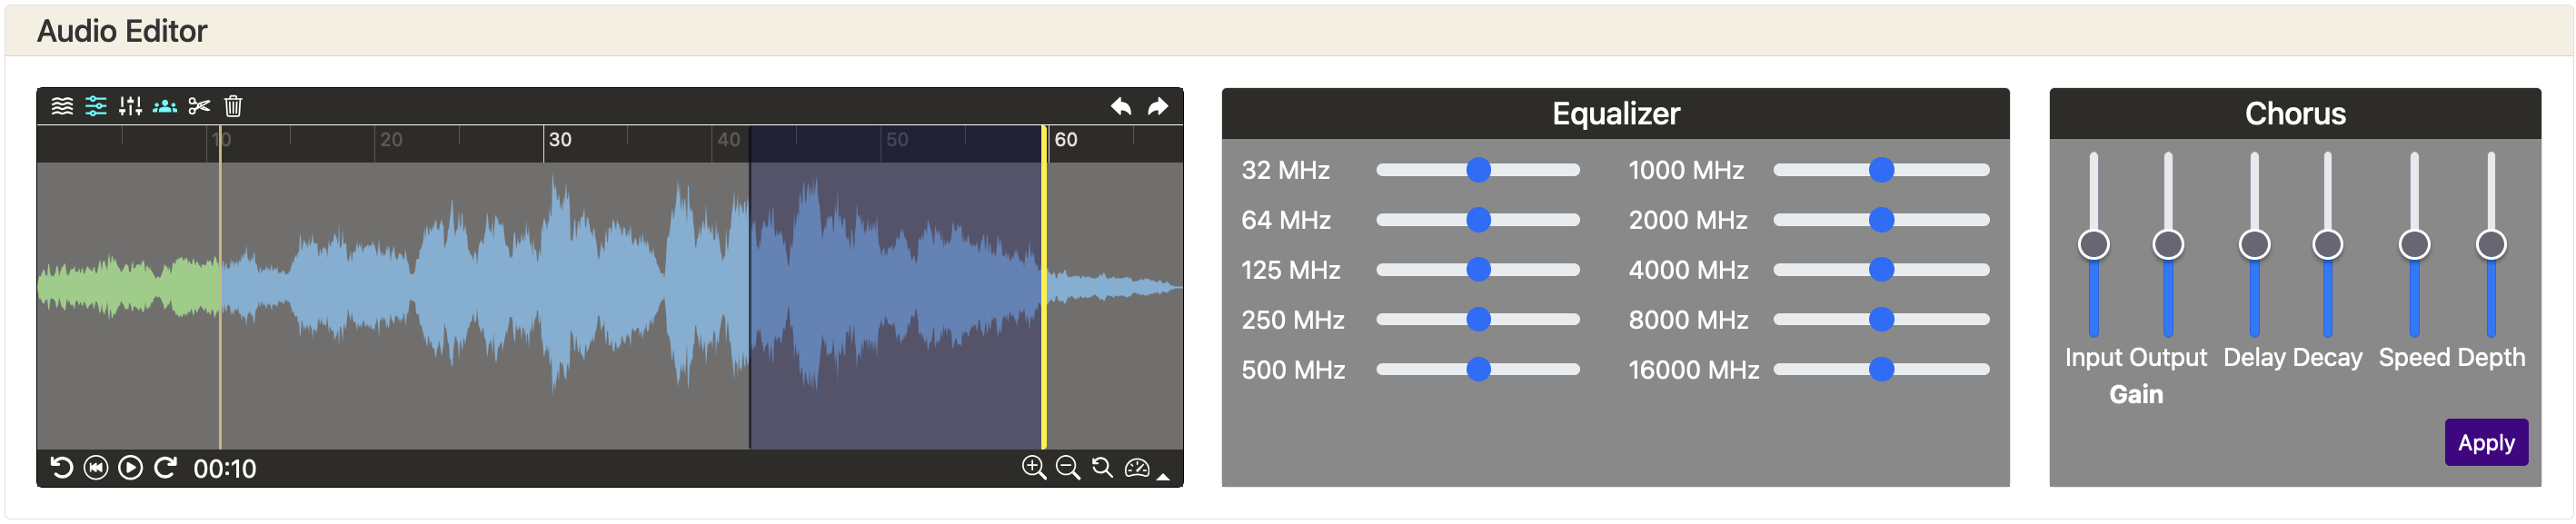
\includegraphics[width=1\linewidth]{proposal//images/features-1.png}
    \caption{Proof of concept custom DAW with several minimum features displayed}
\end{figure}

\subsubsection{`Stretch' Functionality}
Considering the uncertain state of preexisting DAWs and their features, it is worth enumerating some additional `stretch' features and functionality for a custom or extended DAW:
\begin{itemize}
    \item Render split channels.
    \item Extensible UI elements, like effect controllers and widgets
    \item Record directly into the editor via microphone, with live waveform rendering (\autoref{fig:dawrecord}).
    \begin{figure}[H]
        \centering
        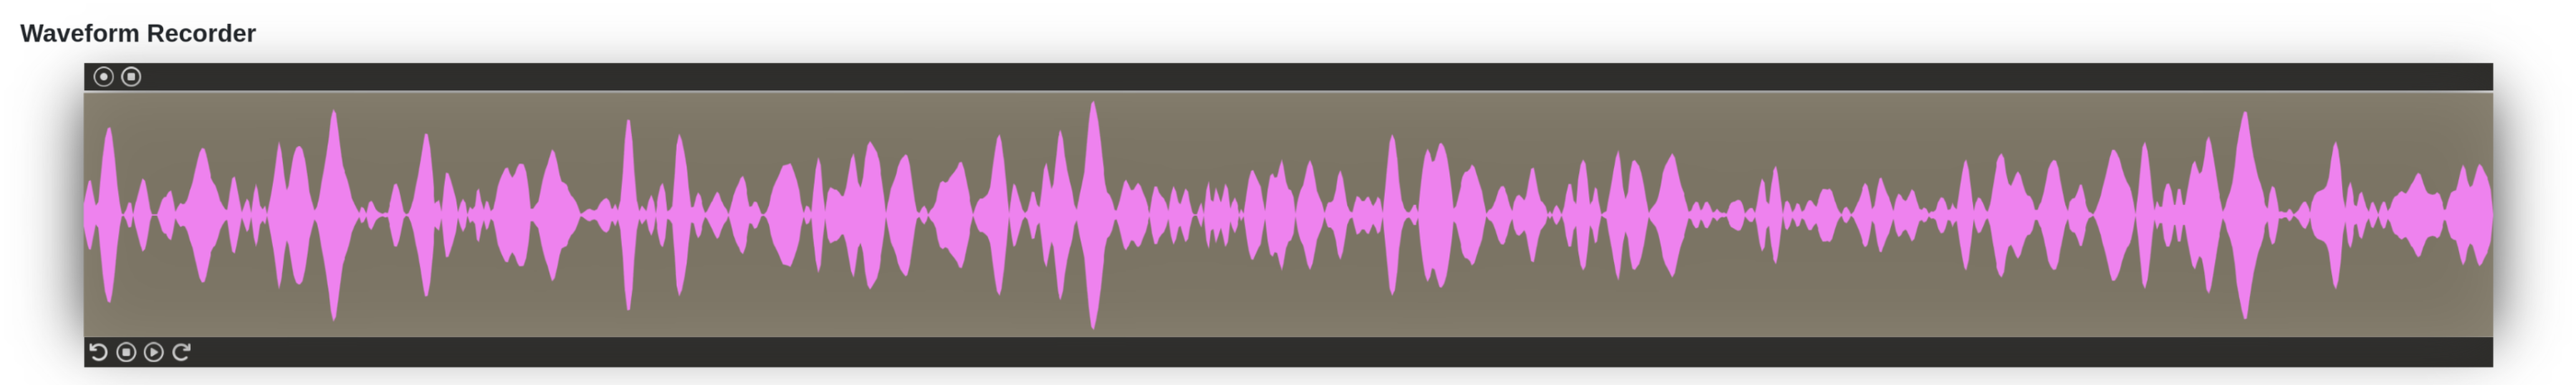
\includegraphics[width=1\linewidth]{proposal/images/daw-recorder.png}
        \caption{Live microphone input waveform visualization}
        \label{fig:dawrecord}
    \end{figure}

    
    \item Ability to apply any of the reverb/chorus/EQ/gain to \textbf{only} a selected region of a clip.
    
    \item A pre-submit check for regions that have dropped audio from recording errors\footnote{Dropped audio in student recordings has been an ongoing issue in MusicCPR, possibly due to student operating system settings.}.
    
    \item Instrument virtualization
    
    \item Additional audio effects:
        \begin{itemize}
            \item Reverb\footnote{Reverb, in contrast to echo, is an effect that simulates a sound in a different space. It can be more difficult to implement because in addition to the input sound, sometimes called a \textit{dry signal}, data is needed about the desired space, called an \textit{impulse response}, to simulate that sample in the space.}
            \item Panning - repositions the source of the sound in the stereo field. 
            \item Compression - increases volume consistency by reducing the difference in volume between the loudest and softest sounds in a sample.
        \end{itemize}
        
    \item Ability to toggle an `envelope' on-waveform (\autoref{fig:dawenvelope})
    \begin{itemize}
        \item An envelope is a tool for controlling clip volume. It can resemble a line graph with nodes overlaid on a waveform. The higher a node is on the waveform, the louder that point in the audio will be.
        \item Nodes can be added and removed with the mouse to change the shape of the envelope; the volume of the clip follows the path of the envelope.
    \begin{figure}[h]
        \centering
        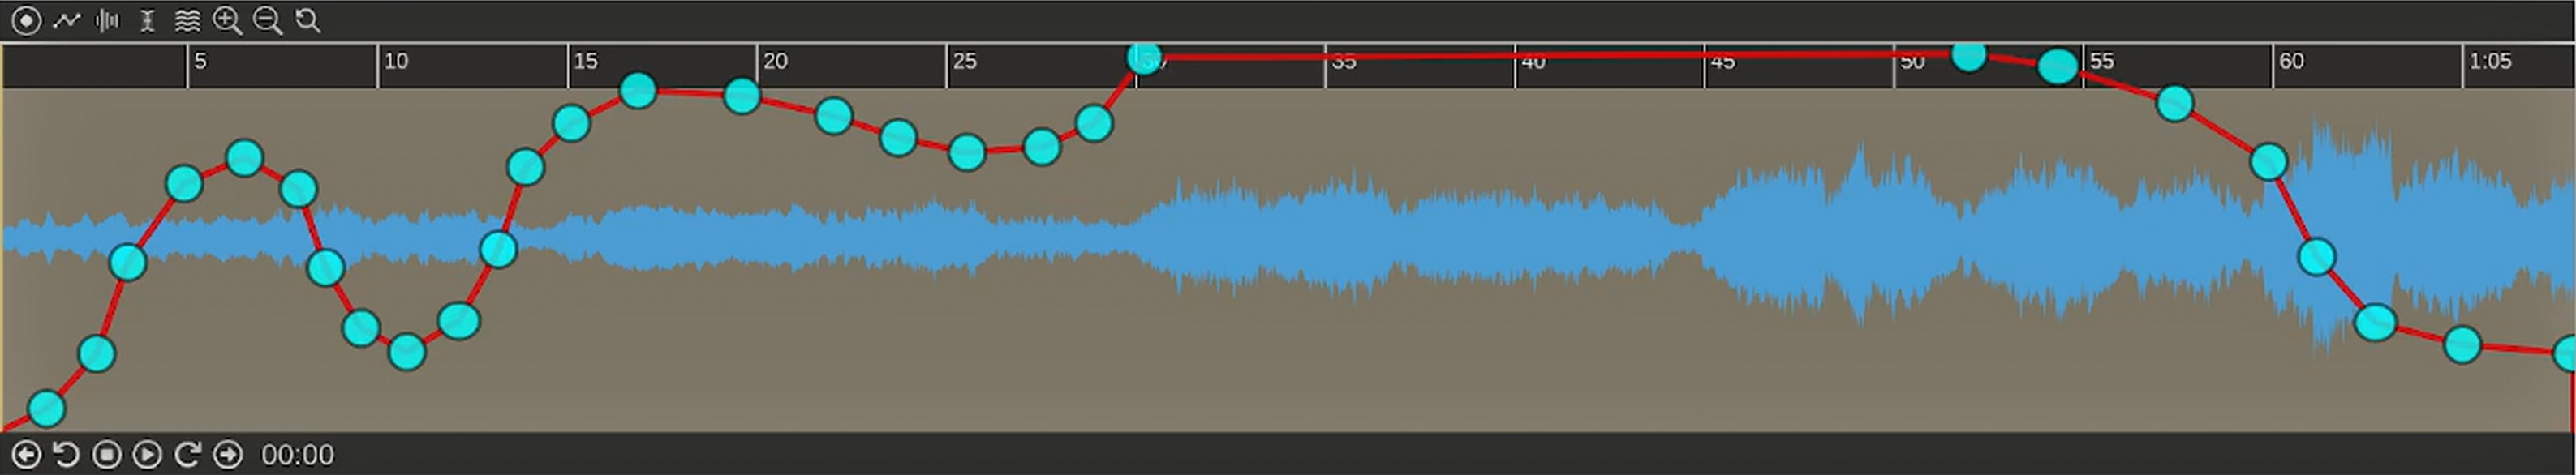
\includegraphics[width=1\linewidth]{proposal/images/daw-envelope-1.png}
        \caption{Proof of concept DAW with envelope on waveform.}
        \label{fig:dawenvelope}
    \end{figure}
    \end{itemize}

    
    \item Ability to hide/show a 2D spectrogram
    \begin{itemize}
        \item A spectrogram is a visual representation of the distribution of an audio signal's frequencies with respect to time and is often represented with heat maps.
        \item If implemented, it will most likely \textit{not} be interactive, unless there is a node module that provides some kind of interactivity with a spectrogram.
        \item The heat map will likely be brightness-based.
    \end{itemize}
    
    \item Ability to toggle a `minimap' waveform (\autoref{fig:dawminimap})
        \begin{itemize}
            \item A minimap is a second, smaller copy of the waveform that can be helpful to see while zoomed in on the main waveform. This is Illustrated in the figure below.
            \item Ideally, it also tracks progress with a cursor and color-coding similar to the main waveform
            \item Consideration should be taken in designing the interface: One could auto-toggle the minimap if it's detected that the user zooms in on the main waveform, but this could be an uncomfortable amount of motion onscreen for some users.
        \begin{figure}[H]
        \centering
            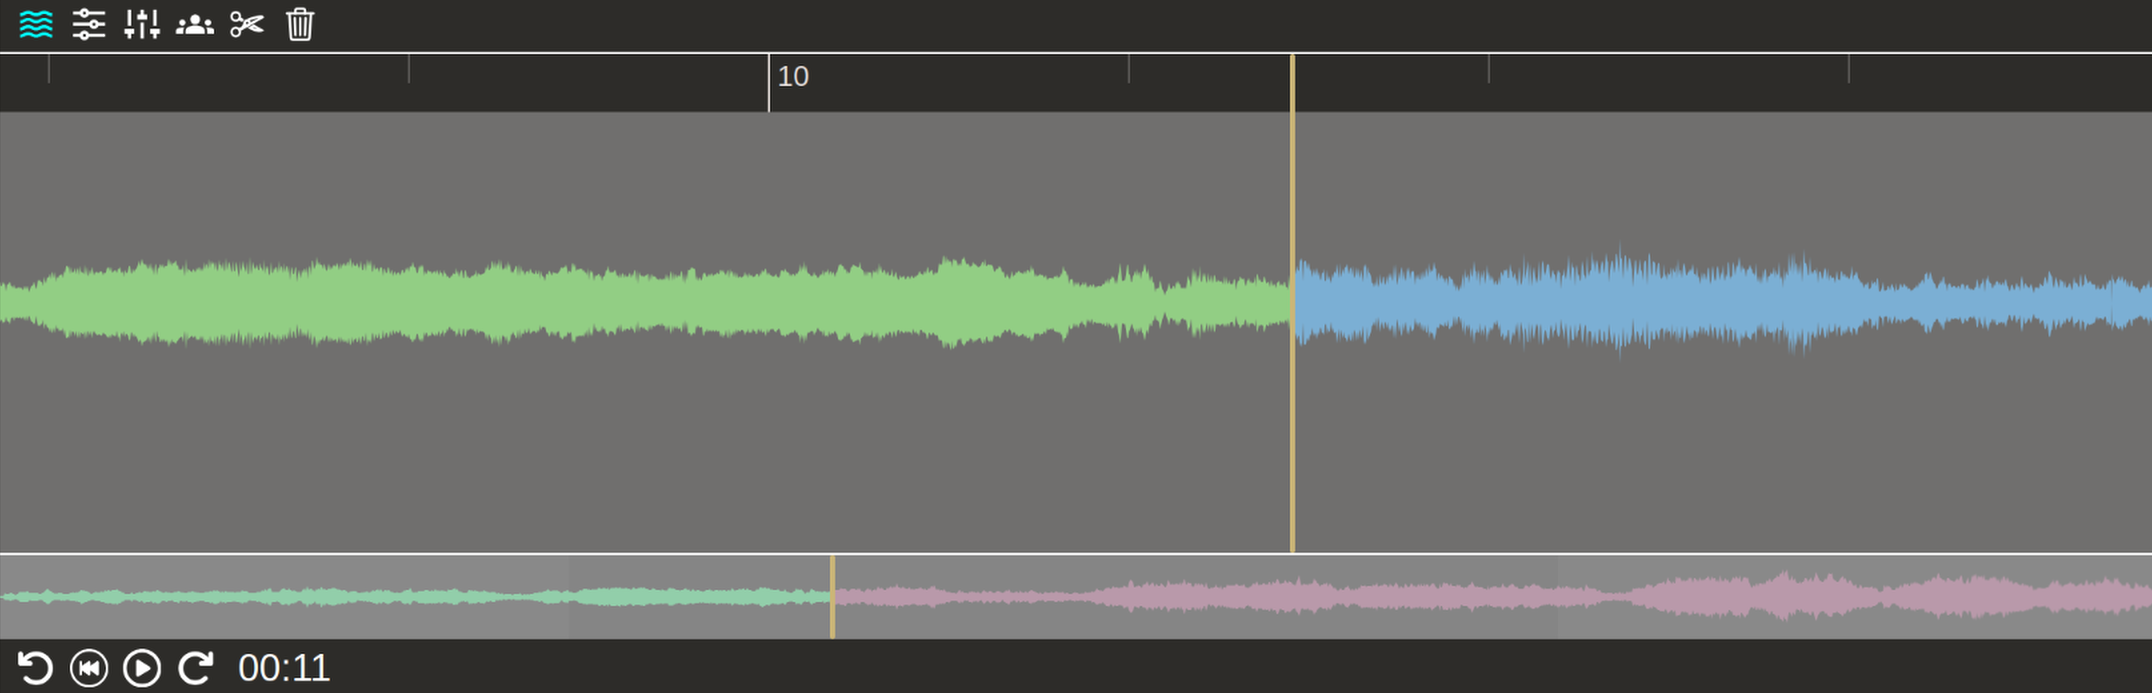
\includegraphics[width=1\linewidth]{proposal//images/minimap-zoom-2.png}
            \caption{`Toggleable' minimap waveform shown (bottom waveform) in the current proof of concept custom DAW component.}
            \label{fig:dawminimap}
        \end{figure}
        \end{itemize}
    
    \item Ability for users to configure the appearance of the DAW as they see fit, e.g., 
        \begin{itemize}
            \item allow users to change and persist custom waveform style/cursor/progress colors, show split channels, default widgets, etc. (Figures \labelcref{fig:default,fig:soundcloud}).
        \end{itemize}
\end{itemize}

\begin{figure}[H]
    \centering
    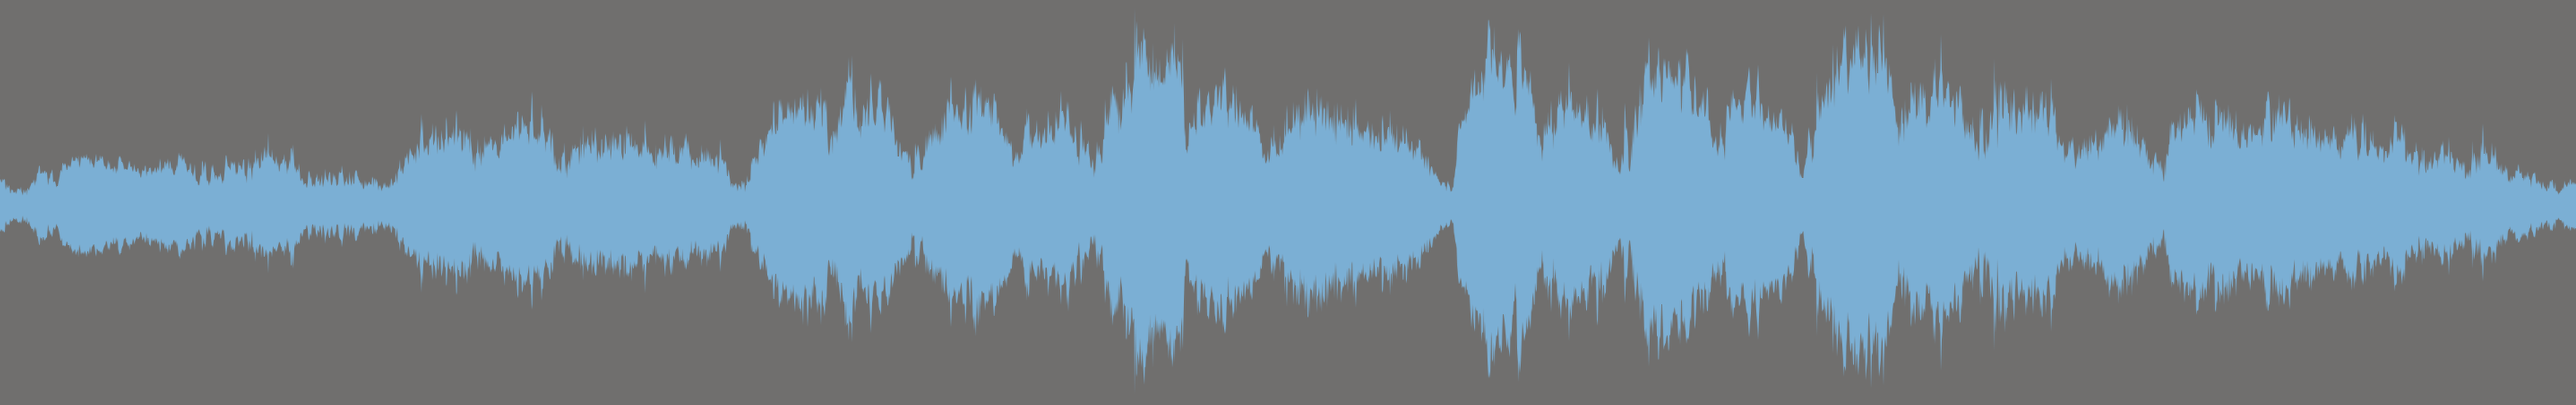
\includegraphics[width=\linewidth]{proposal//images/daw-std-4.png}
    \caption{Default waveform appearance for current DAW proof of concept.}
    \Description[Default waveform appearance for current DAW proof of concept]{The default waveform is continuous unlike the alternative, `bar' style.}
    \label{fig:default}
\end{figure}

\begin{figure}[H]
    \centering
    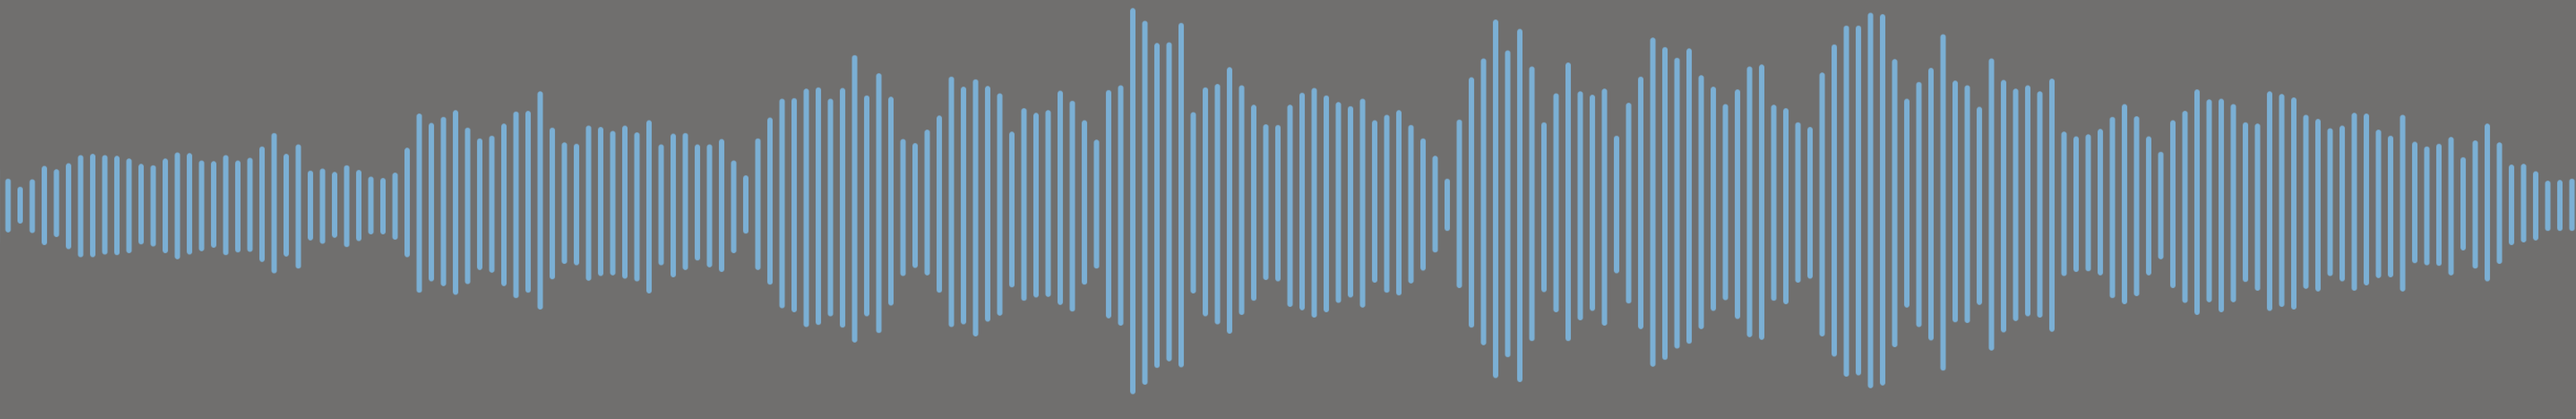
\includegraphics[width=\linewidth]{proposal//images/daw-bars-4.png}
    \caption{Alternative waveform style using `bars' to create waveforms similar to those used on the music streaming platform, SoundCloud.}
        \Description[Alternative waveform appearance for current DAW proof of concept]{This waveform has vertical bars of varying height comprising the waveform. The ends are rounded and there is a slight gap between bars.}
        \label{fig:soundcloud}
\end{figure}

Many of the above stretch features are chiefly quality-of-life issues, and their implementations are not primary goals unless it becomes evident that the absence of one is making DAW use frustrating. When compared to any of the minimum features, certain features like the envelope or spectrogram may be unintuitive and/or distracting for younger students.

\subsection{Hypotheses}
We anticipate that the primary benefits of using a DAW in MusicCPR fall into one of two categories.
The first major grouping of benefits relates to the reduction of strain on IME instructors and mitigation of difficulties posed by modern band integration.
Because of the innumerable challenges that they face in expanding repertoire and acquiring resources, we believe a DAW can act as a convenient, yet powerful facilitating factor for IME instructors' work in modernizing their classrooms.
Modern band programs often call for nonstandard instruments and equipment which are both expensive and difficult to procure for instructors already stretched too thin.
A DAW can not only emulate these instruments, but can do so in ways that forego the technical limitations of the physical instruments themselves, saving instructors additional time spent in individual and group technical instruction. 

The second major grouping of benefits deals with student identity and reducing attrition.
We believe a DAW is akin to a tabula rasa for students to explore and experiment with musical ideas and concepts free from both the influence of standard canon and the fear of judgment from peers and instructors.
Regarding the aforementioned instrument virtualization, we feel that for students who are unsure of or even dissatisfied by their choice of instrument, a DAW can allow them to quickly sample and experience the timbres and textures of a wealth of instruments in a very short amount of time.
This is particularly valuable as expecting elementary school students to guess what instrument they may enjoy playing for their entire pre-college musical education is wholly unreasonable.
We are confident that this workspace will provide a creative outlet and foster the growth of unique musical identities in students otherwise disinterested and musically disenfranchised by the current curriculum.

In addition, student use of such a DAW could have the side effect of improving technological literacy.
Professional DAWs can be overwhelming and intimidating, both in terms of interface and jargon; they are also quite expensive.
Providing a scaled-down DAW can help students build confidence in their abilities to discuss and navigate these complex software systems, preparing them to graduate to larger-scale DAWs if they so choose.

These benefits will advance more than just the goals of the modern band movement.
Realistically, a student may adopt any lens they wish within the DAW, including the standard canon, but also musics considered standard in nations other than the United States.

We anticipate that students of immigrant and refugee families will use MusicCPR to share and preserve their musical heritage while still achieving core artistic goals.
Contrary to the fears of those educators who feel that modern band is a death knell for the WEC, a DAW will expand a student's ability to study and explore all genres, including classical music.


\subsection{Usability Pilot}
Given the possibility we must build a bespoke DAW, the integrity of the primary research will benefit from gathering preliminary research on the workstation user experience.
We chiefly hope to gather data describing whether students are able to complete DAW activities successfully.
If students report non-functionality or difficulties with the interface, we hope to determine the explicit design choices that are causing said issues and resolve them in a subsequent iteration of the DAW.

In addition to functionality, we also wish to ensure that the presentation of the DAW does not detract from usability, namely in the context of web-accessibility.
We also hope to gather opinions about proposed, but unimplemented, quality-of-life features, and whether those features may improve any complaints/barriers-to-use participants may have.
One such unimplemented feature is a menu allowing the user to configure DAW presentation to their liking; this should include cursor color, waveform and progress colors, DAW dimensions, and toolbar and waveform backgrounds at a minimum.
Finally, we wish to establish whether or not the quality of student-submitted recordings changes significantly with the inclusion of the DAW and subsequent student editing.
Ideally, the DAW will have several of the minimum features described above completed prior to the start of the pilot, which we plan for September 2024.


\section{Potential Obstacles \& Facilitating Factors}
There are numerous challenges that building a web-based DAW may present.
Time will need to be allocated for evaluating existing open source web-based DAWs, then ensuring their required scaffolding will work without unwanted side effects for the rest of the MusicCPR platform.

If opting to build a custom DAW, certain existing tools and APIs will likely prove to be indispensable;
we anticipate that two API's in particular will facilitate this task most: the Web Workers API and the Web Audio API.
Historically, browser-based scripting has been bottlenecked by JavaScript's status as a single-threaded programming language.
Given that many standard DAW operations can be computationally expensive, performance with just one thread would likely be intolerable for some users unless other features were sacrificed.
Thankfully, the recent introduction of the Web Workers API allows for multithreading with JavaScript in the browser.
We can thus make use of Worker objects which give us the ability to offload intensive computations and/or longer running tasks in background `worker threads'.
Further, using ``Shared Workers'' will allow us to build a user experience that can span several browsing contexts, if this turns out to be a desirable feature.
Finally, the use of Service Workers may allow us to level the playing field for those students whose networks are slow/unreliable, thanks to its asset caching and request interception.

In addition to the Web Workers API, the recently standardized Web Audio API can facilitate the implementation of certain DAW features such as effect creation, audio visualizations, and many more.
The API will thus make the process of expanding an existing DAW considerably more efficient.
In the event we must build the DAW by hand, the API will likely be crucial to completing the task in an acceptable amount of time. Features and benefits of this API that will help us achieve our goals include:

\begin{itemize}
    \item Processing live audio input.
    \item High-precision, low latency playback for applications that require very precise rhythms.
    \item Automated effect creation and application; effects include envelopes, fades, low frequency oscillation (LFO), and more.
    \item Splitting and merging individual channels of an audio stream.
    \item Spatialized audio and convolution engines for environment emulation
    \item Efficient biquad filtering for popular/commonly used filters
\end{itemize}

\newpage

\section{Implementation Plan}
%  tentative schedule/timeline
\subsection{Summer 2024}
Throughout this project we will continue to review and evaluate the literature to justify the merit of our argument and inform next steps.
In summer of 2024, we will evaluate existing DAWs for compatibility with MusicCPR's current scaffolding and the set of minimum features previously described.
Finally, I will finish and deliver this proposal to my thesis committee.

\begin{center}
    \begin{tabular}{ |p{1cm}||p{6.5cm}|p{6.5cm}| }
    \hline
    \multicolumn{3}{|c|}{\textbf{Summer 2024 Targets}} \\
    \hline
           \textbf{Weeks}
         & \textbf{Tech/Coding}
         & \textbf{Research and Participatory Design} \\
    \hline
            1-2
         &  
             \item Evaluate existing DAW options, keeping compatibility with the Web Audio API and the minimum functionality described earlier in mind
         & 
             \item Continue literature review and proposal drafting
         \\
    \hline
            3-5
         &  
         \begin{itemize}[leftmargin=*]
             \item Scaffold DAW within MusicCPR as proof of concept.
             \item \textbf{If no DAWs meet minimum requirements, begin building custom DAW}
         \end{itemize}
         &
             \item Continue literature review and proposal drafting
         \\
    \hline
            6-8
         &
         \begin{itemize}[leftmargin=*]
             \item If building custom DAW, continue to do so
             \item Otherwise, experiment with adding features to the chosen DAW
         \end{itemize}
        & 
            \item Finalize proposal and present to committee for review
         \\
    \hline
    \end{tabular}
\end{center}

\subsubsection{Status of Targets}
As of August, 2024, I have completed most of the minimum functionality and features of the DAW.
Features which remain to be implemented are:
\begin{itemize}
    \item High, low, and band pass filters
    \item Pre-configured echo, chorus, EQ profiles
    \item Global gain
\end{itemize}

In its current state, the workstation specifically leverages---and relies on---the following tools and libraries: ffmpeg.wasm, Wavesurfer, wavesurfer/react, and the Web Audio API.

Wavesurfer is a library for visualizing audio samples, that is, rendering their waveforms; it is currently the primary means of visual feedback for user manipulations.
There is a library, wavesurfer/react, that attempts to capture some of the Wavesurfer functionality in a Reactive way, though documentation is sparse and only with painstaking experimentation was I able to use it to the benefit of the project.
Wavesurfer was chosen specifically for its myriad plugins and compatibility with the Web Audio API.

Ffmpeg.wasm is a pure WebAssembly/JavaScript port of the popular command line utility, ffmpeg; I currently use it to perform more destructive effects such as cutting regions from an audio sample.
Benefits of using this library include: user edits cause visible changes in waveform, it permits countless different functions, and I am already familiar with many of its commands, so there is less of a learning curve for a time-constrained proof of concept.
It does not currently allow for live feedback on the waveform however; all ffmpeg.wasm effects used thus far must be executed asynchronously.

The Web Audio API was listed as one of two potentially useful tools for completing workstation effects and functionality; it currently is being used for live effects, e.g., edits made with the equalizer widget are audible as they happen.
At the moment manipulations to a source file using Web Audio methods unfortunately do not cause the waveform to change shape live.
Given that Wavesurfer's primary function is to simply \textit{render} a waveform, not \textit{edit} an audio file, and my understanding of how Wavesurfer functions, I do not think wave shaping with live playback reflecting edits is possible. 

It's unclear which approach to user edits is preferred, on one hand, users may appreciate immediate audio feedback to their edits.
On the other, users may gain more utility from being able to \textit{see} the waveform change in response to their edits.
In addition, ffmpeg.wasm operations can be computationally expensive; it's possible however, they may be offloaded to a second thread using a Worker, but it is unclear right now if that functionality will be available with current MusicCPR scaffolding.
In addition to the majority of the minimum requirements, I have also implemented the following `stretch' features:

\begin{itemize}
    \item `Toggleable' minimap
    \item Gain envelope (toggle needs tinkering with, but works statically)
    \item Rendering the waveforms of live microphone data
    \item A utility to scan student audio file submissions for dropped audio regions (the motivation for this described in a footnote on page 6).
    \item `Toggleable' spectrogram (though it takes up a great deal of screen space and offers little interactivity, so it has been scrapped for now)
\end{itemize}

I have styled the DAW using a combination of custom cascading style sheet (CSS) rules along with the frontend framework, React Bootstrap.
The figures referenced earlier in this paper reflect the current style and appearance of the workstation and its widgets.

Prior to the pilot, there are small bugs to fix and accessibility concerns to address; once addressed, I will need to integrate the DAW into the student submission process.
We also may benefit from maintaining logs of individual student edits on audio files, and so I will need to write database models to capture and persist this information.
In addition we must consider options for the `sandbox'/creative DAW mode.



% \pagebreak
\newpage

\subsection{Fall 2024}
During fall of 2024, we will put finishing touches on the DAW in advance of the pilot to be carried out in September at the earliest. If feedback from the pilot indicates changes are necessary prior to starting the study, they should be made at this time. Lastly, we will begin to design the study in preparation for a deployment early in the spring semester. 

\begin{center}
    \begin{tabular}{ |p{1cm}||p{6.5cm}|p{6.5cm}| }
    \hline
    \multicolumn{3}{|c|}{\textbf{Fall 2024 Targets}} \\
    \hline
           \textbf{Weeks}
         & \textbf{Tech/Coding}
         & \textbf{Research and Participatory Design} \\
    \hline
    1-3
    & 
    \begin{itemize}[leftmargin=*]
        \item Incorporate DAW into applicable MusicCPR activities.
        \item Finish DAW `sandbox'
    \end{itemize}
    & 
    Prioritize finishing DAW. \\
    \hline
    4
    &
        Smoke test the DAW.
    &
    Begin to design the study proper:
    \begin{itemize}
        \item Establish methodology; consider:
            \begin{itemize}
                \item Between-subjects design
                \item Pre-post investigation of our research questions
                \item Identify inventories needed to answer said questions
            \end{itemize}
        \item Strategize data collection methods
    \end{itemize} \\
    \hline
    5-7
    &
    \multicolumn{2}{|c|}{\textbf{Conduct pilot}} \\
    \hline
    8-9
    &
    Prioritize pilot data analysis
    &
    Collect and analyze pilot data \\
    \hline
    10-15
    &
    With results of pilot,
    \begin{itemize}
        \item design general workstation improvements
        \item resolve any bugs that arose
    \end{itemize}
    &
    Continue with study design and:
        \begin{itemize}
            \item Identify and recruit subject pool
            \item Plan approaches to data analysis
        \end{itemize} \\
    \hline
    \end{tabular}
\end{center}

% \pagebreak
\newpage

\subsection{Spring 2025}
In the final semester of this project, we will carry out the primary research and I will write my thesis. As the end of the semester approaches, I will plan and practice both my tech demo and presentation. Finally, I will deliver my presentation, and thesis to my committee.

\begin{center}
    \begin{tabular}{ |p{1cm}||p{6.5cm}|p{6.5cm}| }
    \hline
    \multicolumn{3}{|c|}{\textbf{Spring 2025 Targets}} \\
    \hline
           \textbf{Weeks}
         & \textbf{Tech/Coding}
         & \textbf{Research and Participatory Design} \\
    \hline
    1-4
    &
    Monitor Sentry and other points of contact for potential study-breaking bugs/flaws in the DAW and deploy fixes as they are written and tested
    &
    \begin{itemize}[leftmargin=*]
        \item \textbf{Deploy study}
        \item Begin writing the thesis proper, focusing on:
        \begin{itemize}
            \item Introduction 
            \item Literature review
            \item Tables/figures necessary for introductory section
        \end{itemize}
    \end{itemize} \\
    \hline
    5-8
    &
    Continue monitoring for bugs/breaks
    &
    Continue drafting thesis, focusing on:
    \begin{itemize}
        \item Literature review
        \item Methodology
        \item Tables/figures necessary for methodology section
    \end{itemize} \\
    \hline
    9-12
    &
    Prioritize writing
    &
    \begin{itemize}[leftmargin=*]
        \item \textbf{Conclude study}
        \item Continue drafting thesis, focusing on: 
        \begin{itemize}
            \item Results section
            \item Discussion
            \item Tables/figures for methodology and results sections
        \end{itemize}
    \end{itemize}
     \\
    \hline
    13-14
    &
    Start planning tech demo
    &
    \begin{itemize}[leftmargin=*]
        \item Write concluding section and abstract
        \item Begin presentation preparation
    \end{itemize} \\
    \hline
    13-15
    &
    Continue tech demo, making dry runs as ready
    &
    \begin{itemize}[leftmargin=*]
        \item Refine draft with guidance from committee
        \item Continue presentation preparation
    \end{itemize} \\
    \hline
    16-17
    &
    \multicolumn{2}{|c|}{
        \textbf{Deliver presentation}
    } \\
    \hline
    \end{tabular}
\end{center}

%%
%% The acknowledgments section is defined using the "acks" environment
%% (and NOT an unnumbered section). This ensures the proper
%% identification of the section in the article metadata, and the
%% consistent spelling of the heading.
\begin{acks}
To Dr. Weikle and Dr. Johnson, for their endless patience in my delivery of this proposal, Dr. Stewart, for his untiring support and tolerance of my incessant questions, and Dr. Sarah Leventhal, for her input on both early and late drafts of this proposal.
\end{acks}

%%
%% The next two lines define the bibliography style to be used, and
%% the bibliography file.
\bibliographystyle{ACM-Reference-Format}
\bibliography{sample-base}

%%
%% If your work has an appendix, this is the place to put it.
% \appendix

% \section{Dr. Stewart's Notes}

% two main things Stewart would say about DAW for MusicCPR: (1) "classical" musicians need these skills and these needs are currently neglected in general, and (2) there are (new) genres of music that require at least some if not quite a lot of digital music production

% \begin{itemize}
%     \item fewer students than ever in IME
%     \item IME as hegemonic/canon-clutching as ever
%     \item students have a hard time feeling like they belong in the
%         \begin{itemize}
%             \item IME classroom
%             \item field of music performance
%             \item like their culture or musical interests are relevant/legitimate
%         \end{itemize}
%     \item lifelong musicians will need to know as early as high school how to publish/mix their music, and many rely on some nerd friend who was never actually taught either, this is hidden curriculum and a barrier to the least advantaged
% \end{itemize}

% \begin{enumerate}
%     \item diversity of repertoire available/legitimized in formal IME
%     \item intentional focus on technological literacy should improve individual musician self-efficacy with respect to "publishing", sharing, getting feedback, experimenting?
%     \item By integrating digital music production skills in IME, we may be able to leverage the only legitimate path to studying music in public education to also support students who would like to diverge from western classical to other genres/traditions
% \end{enumerate}

\end{document}
\endinput
%%
%% End of file `sample-authordraft.tex'.
